%\documentclass{article}

%\usepackage[utf8]{inputenc}
%\usepackage[T1]{fontenc}      
%\usepackage[francais]{babel}
%\usepackage{graphicx}
%\usepackage{circuitikz}
%\usepackage[squaren, Gray]{SIunits}
%\usepackage{sistyle}
%\usepackage[autolanguage]{numprint}
%\usepackage{pgfplots}
%\usepackage{amsmath,amssymb,array}
%\usepackage{url}
%\usepackage[version=3]{mhchem}
%\usepackage{array} 

%\begin{document}
%%%%%% titlepage.tex %%%%%%


%\begin{titlepage}
%
%\begin{center}
%
%\textsc{\Large Université Catholique de Louvain}\\[0.5cm]
%\textsc{\Large \'Ecole Polytechnique de Louvain}\\[1cm]
%
%{\Huge \bfseries Projet}\\[0.15cm]
%
%%%\begin{center}
%%%\includegraphics[width = 8cm]{./titlepage/BARRA.jpg}
%%%\end{center}
%
%\rule{\linewidth}{0.3mm}\\[0.1cm]
%{\huge \bfseries Rapport de tache 1}\\[0.02cm]
%\rule{\linewidth}{0.3mm}\\[0.5cm]
%
%{\LARGE \bsc{Groupe} 1}\\[1cm]
%
%\begin{minipage}{0.5\textwidth}
%\begin{flushleft} \Large
%\emph{Auteurs:}\\
%\Large Simon \textsc{Boigelot} \normalsize 75971300\\
%\Large Virgile \textsc{Goyens} \normalsize 83391300\\
%\Large Corentin \textsc{Joachim} \normalsize 75971300\\
%\Large Xavier \textsc{Lambein} \normalsize 54621300\\
%\Large Edward \textsc{Nicol} \normalsize 27101300\\
%\Large Léa \textsc{Paulus} \normalsize 48251100\\
%\Large Abbas \textsc{Sliti} \normalsize 75971300
%\end{flushleft}
%\end{minipage}
%\begin{minipage}{0.4 \textwidth}
%\begin{flushright} \large
%\emph{Cours:} \\
%LFSAB1503\\
%\emph{Professeurs responsables:} \\
%J. De Wilde \\
%P. Luis Alconero \\
%D. Mignon \\
%\emph{Assistant:} \\
%*** \\
%\end{flushright}
%\end{minipage}
%
%\vfill
%
%%%\begin{minipage}{0.3\textwidth}
%%%\begin{flushleft}
%%%\includegraphics[height=2.5cm]{./titlepage/logo-ucl.jpg}
%%%\end{flushleft}
%%%\end{minipage}
%\begin{minipage}{0.3\textwidth}
%\begin{center}
%{\large FSA12BA}\\
%{\large 21 septembre 2014}
%\end{center}
%\end{minipage}
%%%\begin{minipage}{0.3\textwidth}
%%%\begin{flushright}
%%%\includegraphics[height=1cm]{./titlepage/logo-epl.jpg}
%%%\end{flushright}
%%%\end{minipage}
%
%\end{center}
%
%\end{titlepage}


\section{Bilan de masse}

L'équation de la production d'ammoniac selon le procédé Haber-Bosch est la suivante: 

$$\ce {N2 + 3H2 -> 2NH3}$$

Nous voulons calculer la quantité de réactifs pour obtenir une quantité de \unit{1000}{\tonne} d'ammoniac. Pour cela avec les masses molaires respectives de \unit{28}{\gram/\mole} et \unit{2}{\gram/\mole} du diazote et du dihydrogène, il nous faut: 
\begin{center}
 \begin{tabular}{|l|c|r|}
   \hline
    & dihydrogène & diazote \\
   \hline
   Nb mole & $88.2\cdot 10^6$ & $29.4\cdot 10^6$ \\
   Poids & \unit{176.8}{\tonne} & \unit{823.2}{\tonne}  \\
   \hline
 \end{tabular}
\end{center}

Notre bilan de masse est maintenant fini.

\section{Aspect thermique}

Nous devons faire en sorte que notre réacteur soit à une température constante de \unit{500}{\celsius}. Étant en présence d'une réaction exothermique, pour le refroidir, nous disposons d'un flux d'eau dont la température varie entre \unit{25}{\celsius} et \unit{90}{\celsius}.


Nous utilisons comme hypothèses que le réacteur est, au départ, à \unit{500}{\celsius} et que la réaction se fait en continu.


On sait que la réaction dégage \unit{92.22}{kJ/\mole}, on considère que l'eau est injectée à \unit{25}{\celsius} et qu'une fois qu'elle atteint la température de \unit{90}{\celsius} elle ressort du circuit. 
Il nous est donné dans des tables qu'à l'état liquide, l'eau a une capacité calorifique \unit{75.29}{\joule/\kelvin \cdot \mole}. Ayant une différence de température de \unit{65}{\celsius} entre l'entrée et la sortie nous obtenons l'expression suivante:
$$ 75.29\cdot 65 \cdot x = 92.22\cdot 10^3 \cdot 58.8 \cdot 10^6,$$
avec $x$ le nombre de mole \ce{H_2 O} nécessaire.

Nous trouvons qu'il nous faut $\unit{738687}{m^3/jour}$ pour refroidir la production de \unit{1000}{\tonne} d'ammoniac. Cela est équivalent à un débit de $\unit{205}{m^3/\second}$.



\section{Provenance des réactifs}
 
Pour ce qui est de la provenance des réactifs plusieurs options ont été considérées. Pour ce qui est de l'eau nous avons pensé utiliser l'électrolyse de l'eau ainsi que la décomposition thermochimique. Pour le diazote nous avions pensé utiliser le procédé Lindé qui consiste en une distillation de l'air liquide.

Cependant ces processus étant coûteux et l'air étant composée à 78.1\%, nous avons opté pour l'hydrogénation du \ce{N_2(g)} atmosphérique par le \ce{H_2(g)}. 

Un flow-sheet de notre procédé ce trouve à la figure~\ref{Flowsheet}.
\begin{figure}
  \begin{center}
 	 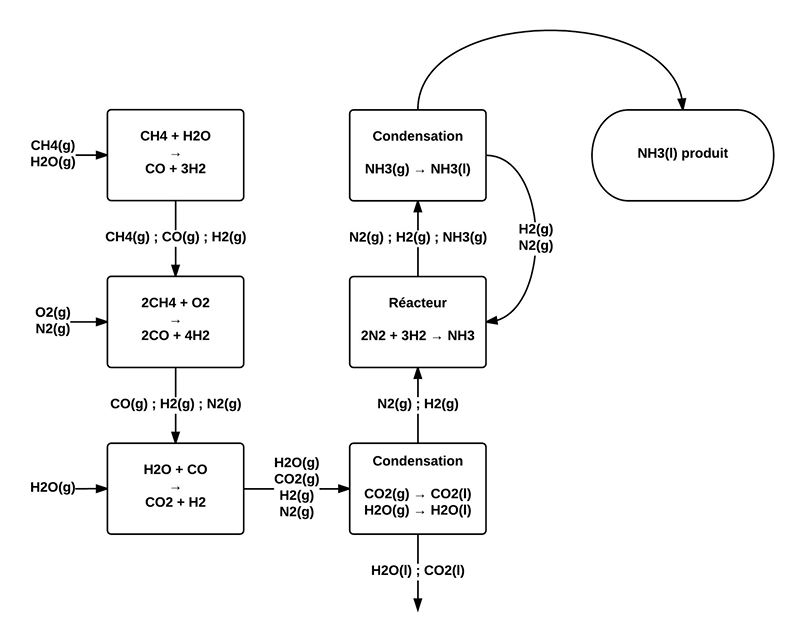
\includegraphics[scale=0.4]{Shema1.jpg}
  	 \caption{Flow-sheet}
  	 \label{Flowsheet}
  \end{center}
\end{figure}


%\end{document}
